\section{Real-time Visualization} (0.5 page) (AJ, JP)
\label{sec:vis}

To enable our focus and context transparent rendering, we employ an A-buffer to acquire a list of participating fragments.
These fragments represent three types of surface patches, computed in previous steps, analytically computed for a given ray.
This is obtained via an analytical approach.
%We implemented the A-buffer using per-pixel linked lists~\cite{yang2010real}, since our main focus was on extending the CB algorithm to enable the extraction of different surface components.
%The current A-buffer method can be easily swapped to benefit from, e.g., 

\subsection{Rendering of spherical patches}
\label{sec:spherical-patches}

A sphere can form an arbitrary number of spherical patches which may lie in different surface components.
To enable individual visualization of surface components, e.g., different coloring, transparency or visibility, we ray-cast each spherical patch as a separate surface primitive.
This way, we are able to visually distinguish between different surface components.

The sides of a spherical patch are formed by small circle arcs.
We apply the odd-even rule for polygons \cite{shimrat1962algorithm} to test whether a point lies inside a patch.
Firstly, we compute intersection points $P_{front}$ and $P_{back}$ of a ray with patch's sphere.
We describe the point in patch test only for $P_{front}$ calling it $P$, as the same test is applied also to $P_{back}$.
Before the application of the odd-even rule, we choose a point $O$ lying outside the patch.
Then, we test line $OP$ (shortest path on a sphere) for intersection with each side (small circle arc) of the patch.
The intersection of a line $OP$ with a small circle arc is computed in two steps (see Figure~\ref{fig:spherical-patch}):
\begin{enumerate}
  \item The intersection of the circles containing the line and the arc is computed --- they can intersect in 0 to 2 points.
  \item The intersection points are tested whether they lie on the line and the arc.
\end{enumerate}
Finally, the number of intersections with all sides is summed and if it is even then the point lies inside the patch.

\begin{figure}[htp]
  \centering
  \begin{subfigure}[c]{0.52\columnwidth}
    \centering
    \includegraphics[height=1.9in]{image/patch.png}
    \caption{%Point in spherical patch test.
		The intersection $I_1$ lies on an intersection line between two planes containing arcs $OP$ and $AB$.}
		\label{fig:spherical-patch}
  \end{subfigure}%
  \quad
  \begin{subfigure}[c]{0.44\columnwidth}
    \centering
    \includegraphics[height=1.6in]{image/outer.png}
    \caption{%A torus formed by carbon ($C_C$) and hydrogen ($C_H$) atoms.
		The center of the torus ($C_{t}$) lies outside the atom centers, while the center of its visibility sphere $C_{vs}$ lies between $C_C$ and $C_H$.}
		\label{fig:outer-point}
  \end{subfigure}
\caption{Point in spherical patch test (a). A torus formed by carbon ($C_C$) and hydrogen ($C_H$) atoms (b).}
\end{figure}

Differently from the planar case, the point $O$ has to be specified for the algorithm to be correct.
%Otherwise, we would count intersections of patch's sides with a great circle containing $P$.
%Then, the intersection count would be the same regardless of $P$ being inside or outside the patch, making the rule inapplicable.
We compute $O$ by intersecting a patch's sphere by an axis of one (arbitrary) of its delimiting tori.
This way, we get two intersection points from which we choose the one that lies in the direction of the torus's visibility sphere (see Figure~\ref{fig:outer-point}).

\subsection{Opacity Mapping}
Borland~\cite{borland2011ambient} proposed to utilize ambient occlusion (AO) values to alter the opacity. Motivated by his approach, we exploit the ambient occlusion values as well. Since, we would like to maintain fast rendering performance, we need to remedy the issue of having an object space technique to evaluate the AO values. In the former work of Borland, the performance was not an important factor, which allows him to exploit the full object space AO evaluation. Here, we opted for the most recent approach, proposed by Grottel et al.~\cite{grottel2012object}, which renders ambient occlusion values to a $3D$ grid containing an estimate of the volume area of atoms located inside a voxel. Although this approach only reflects the volume of atoms and not the molecular surface, we find it as a good trade off between the visual precision and the performance measure taking into consideration that these values are not employed directly, but as opacity modulators instead.
	
\begin{figure}[htb]
\centering
  \includegraphics[width=0.8\columnwidth]{image/ray_fragments.png}
  \caption{(TODO make more nice with overlay AO grid). An example of the list of fragments per a given ray. The color of the circles represent the obtain ambient occlusion value.}
	\label{fig:ray_fragments}
\end{figure}

Interactive Analysis (0.5 page) (ALL)
\begin{itemize}
  \item Possibilities (scenario, dynamics, pipeline)
  \item Feedback
\end{itemize}

\subsection{Cavity area estimation}

We enhance the visualization of cavities by coloring their surface by their approximate area.
To estimate the area, we sum areas of all triangles that form the cavity surface.
The area of a spherical triangle is calculated as follows:

\begin{equation}
  S = r_{probe}^2 \left[ \left( A + B + C \right) - \pi \right],
\end{equation}

where $A$, $B$ and $C$ are angles of the triangle. We do the area computation in a GLSL compute shader which computes areas of individual triangles and sums them using atomics.

We decided to neglect areas of spherical and toroidal patches since from our observations their influence on the exact cavity area is much smaller compared to triangles.
%Therefore, the cavity area we compute is \textcolor{red}{underestimated -- maybe an equation?}.
Of course, this observation does not hold for the molecular surface.
%\textcolor{red}{What about coloring?}
